%!TEX encoding=UTF-8 Unicode
%!TEX root=../tabarnac.tex

\section{TABARNAC}
\label{sec:design}

\TABARNAC is divided into two parts: the instrumentation tool and the
visualization. In this section, we discuss the implementation of both parts.

\subsection{Instrumentation}
\label{sec:design-impl}

The instrumentation part of \TABARNAC is based on a custom memory tracer for
the Pin dynamic binary instrumentation tool~\cite{Luk05Pin}, although pin is
an Intel technology, it works also on AMD processors
\DB{If enough space, speak about slowdown on AMD \ldots} .
Before running the application, our tool retrieves static memory allocation
information using the \texttt{libelfg0} library. Dynamic allocations are
intercepted with a \texttt{malloc} replacement. If the application is
compiled with debug flags~(\texttt{-g}), the structure names that are malloced can be extracted from the source
code. Finally, each time a thread is created, we compute
its stack bounds, and create a virtual structure named \texttt{Stack\#N} where
$N$ is the thread id. Only structures that are bigger than one page (usually
$4$Kib in current x86\_64 architectures) are recorded as our
analysis granularity is the memory page. The data structure informations (name,
size and address) are not used during the instrumentation, they are only
printed in a file at the end of the analysis to be used by the visualization
tool.

During the execution, every memory access of the parallel application is traced.
For each access, we store the type of access (read or write), the memory page that was accessed, and the thread ID.
The information is stored on a per-thread basis, as shown in
Listing~\ref{lst:mem}, making the code completely lock-free, as well as minimizing the amount of false sharing between threads.

%\begin{figure}[!h]
\begin{lstlisting}[caption={Code executed on each memory access. The \texttt{address}, \texttt{threadid} and \texttt{type} parameters are provided by Pin.},label=lst:mem]
	void mem_access(unsigned long address, int threadid, char type)
	{
		uint64_t page = address >> page_bits;
		acc[threadid][page][type]++;
	}

\end{lstlisting}
%\caption{Code that is executed on each memory access.}
%\label{fig:code}
%\end{figure}


After tracing finishes, we generate three \texttt{csv} files.  The first file
contains the list of pages and the number of reads and writes per thread. The
second file contains the list of structures with their names, sizes and start
addresses, finally the third contains the stacks size and addresses.
We then call an R-markdown script which reads the \texttt{csv} files,
retrieves the page / data structure mapping and generates the final
visualization presented in the next subsection.

% not relevant I'd say:
% \TABARNAC have very few dependencies and can be installed easily. If all the R
% library required to generate the visualization are not present, our tool is
% able to install them automatically. By default \TABARNAC generate the memory
% trace and the visualization, but the user can also choose to only generate the
% memory trace or the visualization. This is useful for people who cannot
% install R on the machine used to generate the trace. Moreover it allows the
% user to customize the plots generate by the R script.

\subsection{Visualization}
\label{sec:design-visu}

Providing an easy to analyze visualization of a memory trace is a challenge. We
opted for an assisted visualization. Once the analysis phase is done,
\TABARNAC generates the visualization (as an HTML page), providing a summary
of the trace through several plots\footnote{A full example is available at
    \url{http://dbeniamine.github.io/Tabarnac/example}}. Each plot is introduced by an explanation
of its presentation, what common issues it can help to understand and provides
suggestions on how to fix these issues.  The visualization starts with a small
introduction, recapitulating the main principles while developing for NUMA
machines, and shows the hardware topology of the analyzed machine extracted
with Hwloc~\cite{Broquedis10hwloc}.

In the next part, the visualization focuses on the usage of data structures. Some
structures might be ignored for two reasons: either no accesses have been
detected during the analysis, which happens for structures used by external
libraries, or less than 0.01\% of the total accesses happens on them. This is
done to make the output more readable. However, it is possible to ask
\TABARNAC not to ignore structures in the second case for a more detailed view.

\begin{figure}[htb]
    \centering
    \subfigure[Size of structures (pages).]{
        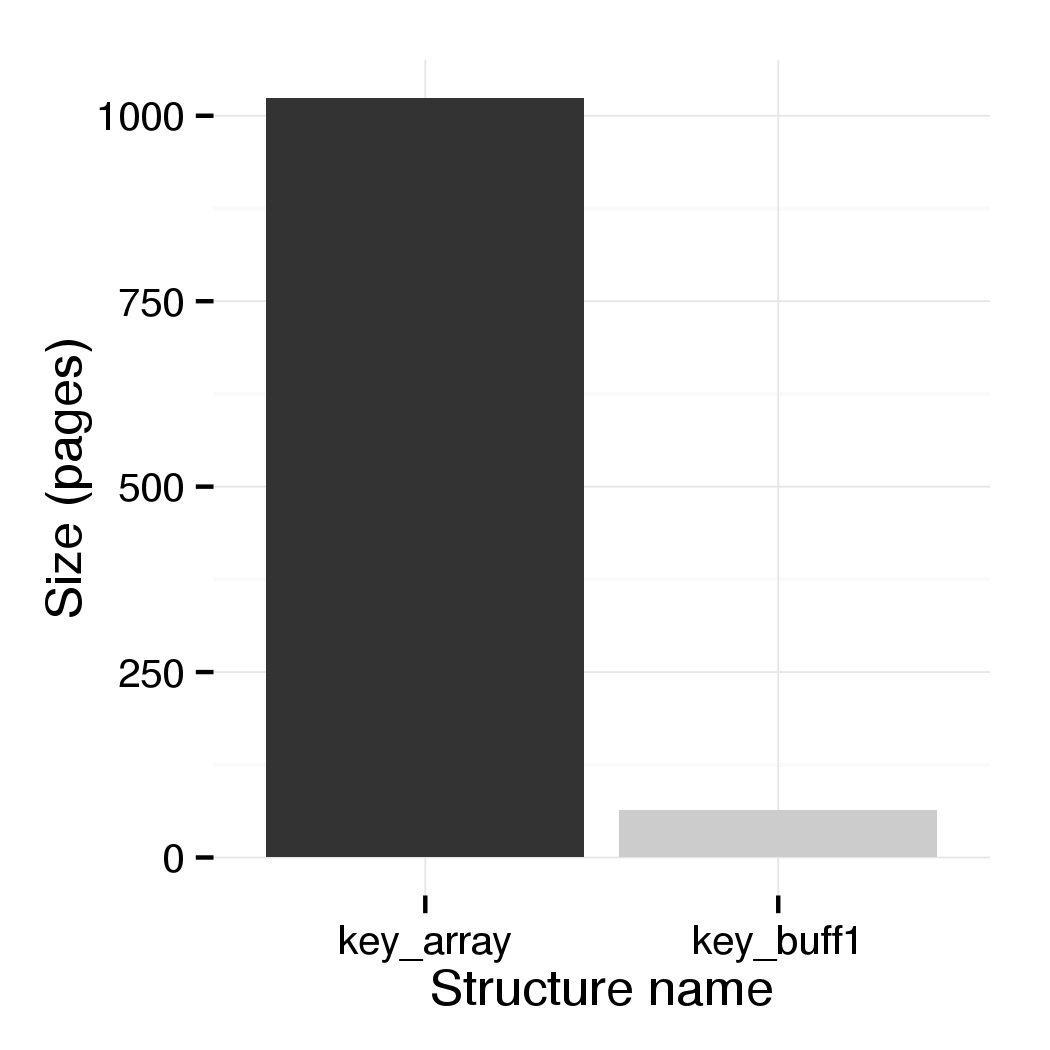
\includegraphics[width=.45\linewidth]{example_sz}
        \label{fig:example_sz}
    }
    \subfigure[Number of Read and Write per structure.]{
        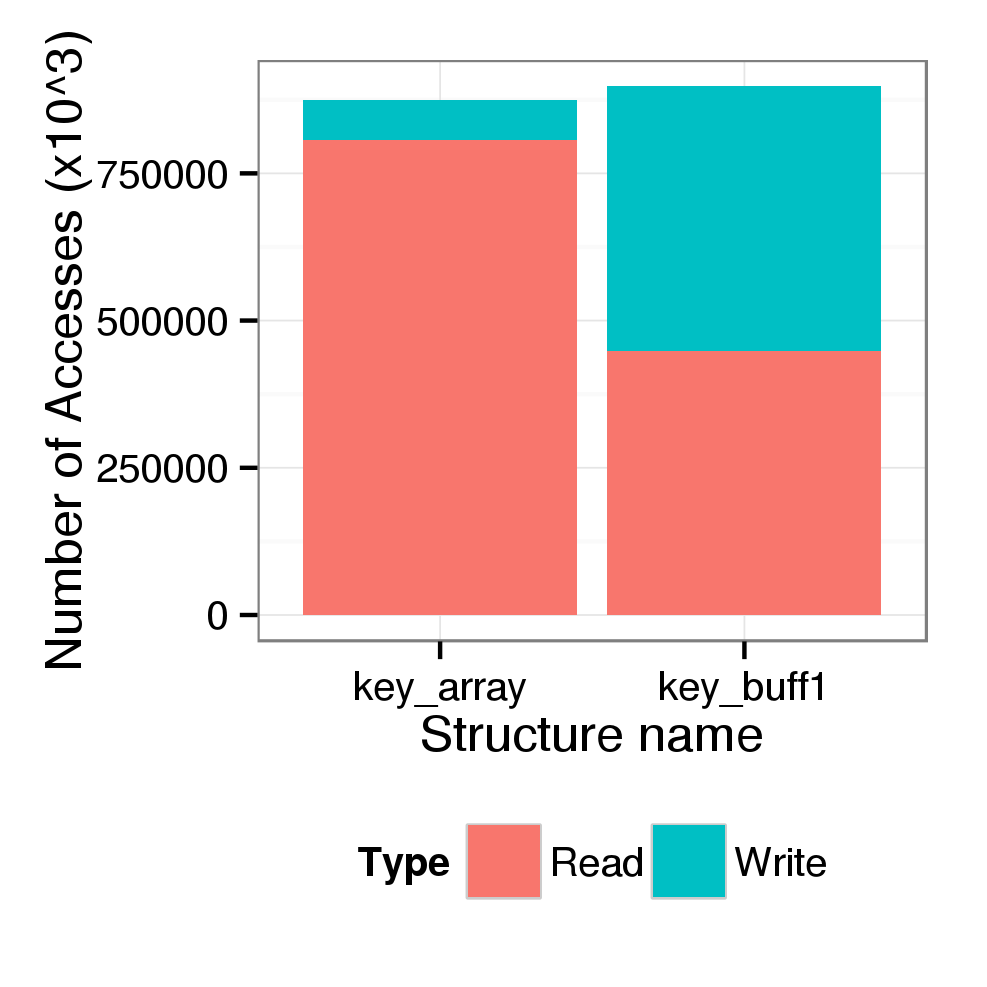
\includegraphics[width=.45\linewidth]{example_rw}
        \label{fig:example_rw}
    }
    \subfigure[Access distribution.
%    Each point represents the number of access to one page done by one thread.
    ]{
        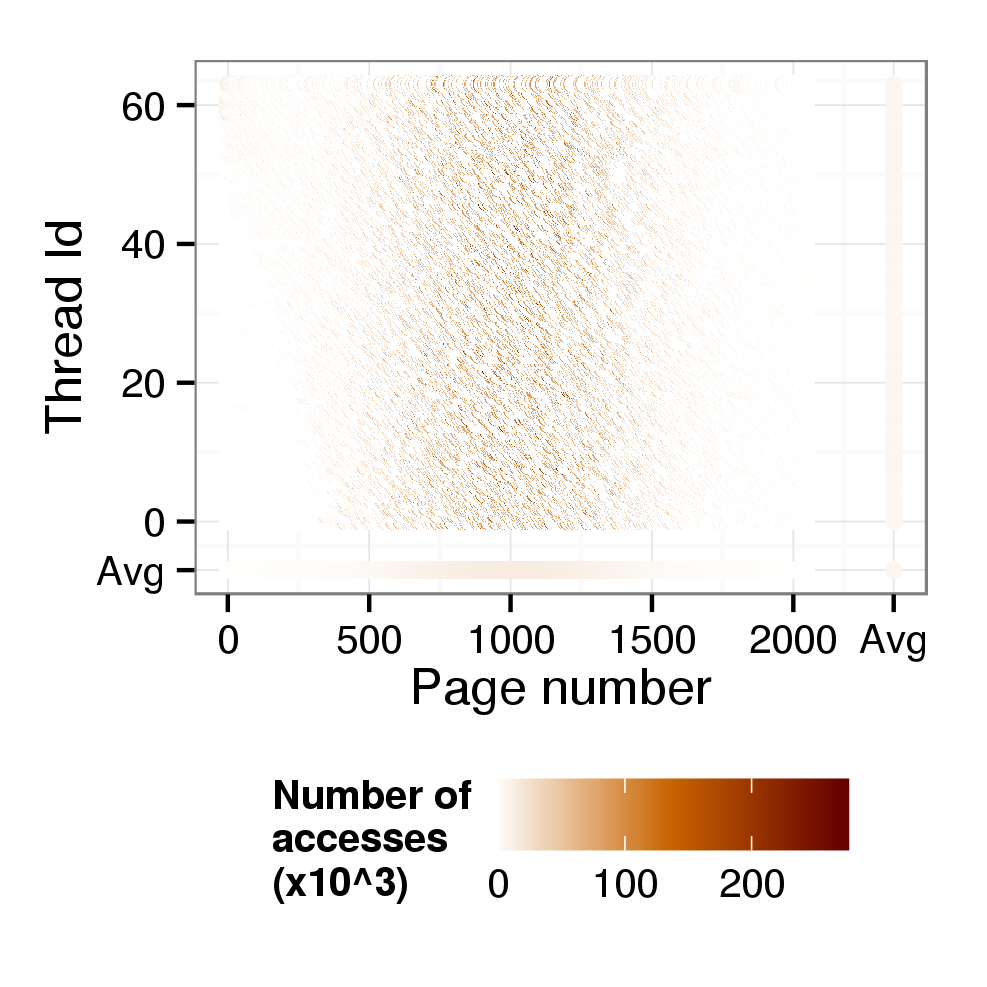
\includegraphics[width=.45\linewidth]{example_dist}
        \label{fig:example_dist}
    }
    \subfigure[First touch distribution.
%   Each point shows which thread is responsible of the first access on one page.
    ]{
        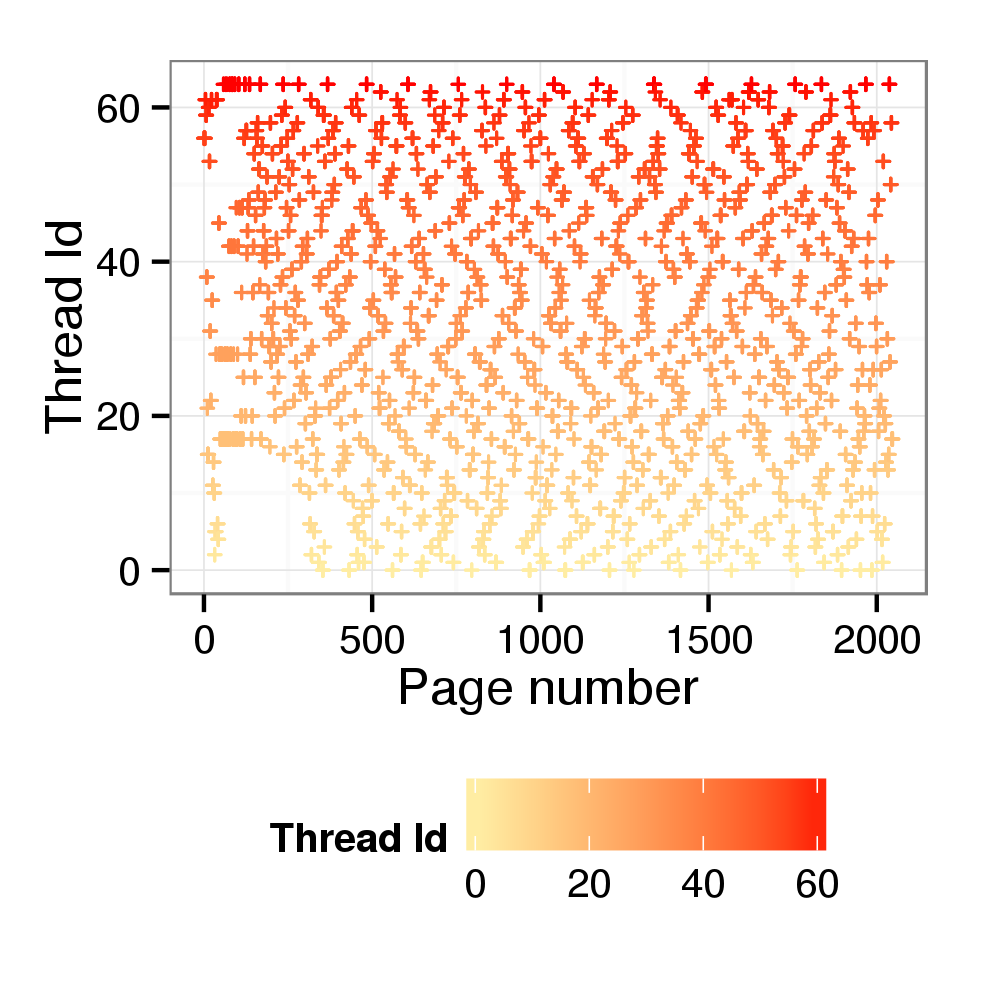
\includegraphics[width=.45\linewidth]{example_ft}
        \label{fig:example_ft}
    }
    \label{fig:example_plot1}
    \caption{Example plots from \TABARNAC.}
\end{figure}

The first series of plots presents information concerning the relative
importance of the data structures. It consists of two plots, showing first the
size of each data structure, as in Figure~\ref{fig:example_sz}, then the
number of reads and writes  on each structure (Figure~\ref{fig:example_rw}). These plots give a
general idea of the structures used by the parallel application.
Moreover, knowing the read/write behavior is very
useful as it determines the possible optimizations. For instance, structures
written only during initialization (or very rarely) can be relatively easily
duplicated, such that each NUMA node works on a local copy.

The second series of plots is the most important one. For each structures, it
shows the density of access done by each thread over the structure and the
global distribution. As we can see in Figure~\ref{fig:example_dist}, there is
one line per thread, the darker is the line the more the thread accessed the
page. It gives an easy way to understand the data sharing between threads and
the usage of structures. They can be used to identify inefficient memory usage
and to determine the best NUMA mapping policy.

%\begin{figure}[htb]
%    \centering
%    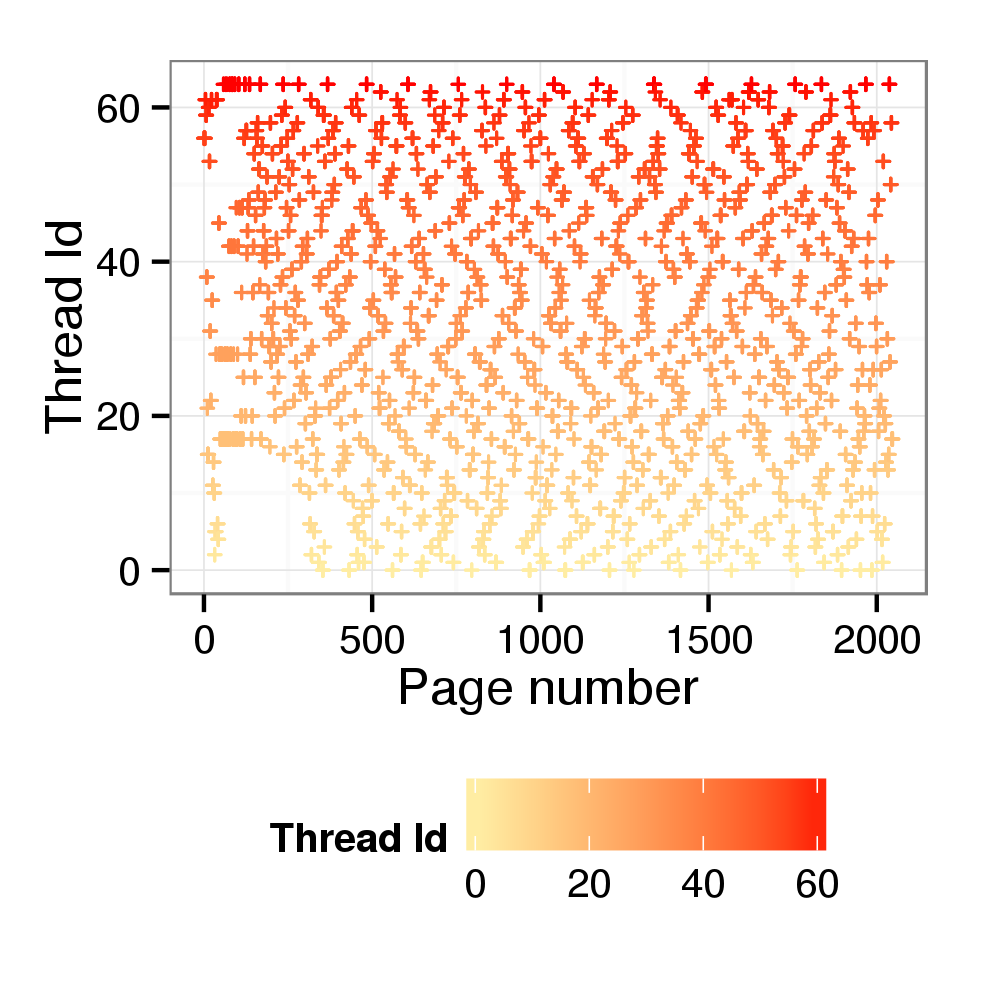
\includegraphics[height=.2\textheight]{example_ft}
%    \caption{Example of first touch distribution Each point show which thread
%    is responsible of the first access on one page.}
%    \label{fig:example_ft}
%\end{figure}


Finally, \TABARNAC provides a plot that shows for each page of each structure
which thread was responsible for the first touch
(Figure~\ref{fig:example_ft}). This information is important as the
default policy for \emph{Linux} and most other operating systems is to map a page as close as possible to the first
thread accessing it. If the first touch distribution does not fit the actual
access distribution, the default mapping done by \emph{Linux} might not be
efficient. To improve this issue, the developer can either correct the first
touch or do some manual data mapping to ensure better memory access locality
during the execution.
